\documentclass{standalone}

\usepackage{tikz}

\begin{document}
\Large
\begin{tikzpicture}
% \draw[help lines, black!30] (0,0) grid (25,12);
\draw[line width=0.5mm, black] 
    (0,0) rectangle (12,12);
\draw[line width=0.5mm, blue, fill=blue!25, rounded corners=2mm] 
    (0,0) ..controls+(1,0.4).. 
    (2,0) ..controls+(0,6).. 
    (4,12) ..controls+(-1,-0.4).. 
    (2,12) ..controls+(0,-3).. 
    (0,6) ..controls+(1,-3).. cycle
    (4,0) ..controls+(2,6).. 
    (6,12) ..controls+(-2,-6).. cycle
    (6,0) ..controls+(2,6).. 
    (8,12) ..controls+(-2,-6).. cycle
    (12,12) ..controls+(-1,-0.4).. 
    (10,12) ..controls+(0,-6).. 
    (8,0) ..controls+(1,0.4).. 
    (10,0) ..controls+(0,3).. 
    (12,6) ..controls+(-1,3).. cycle;
\fill[red] foreach \a in 
    {(0,0), (2,0), (4,0), (6,0), (8,0), (10,0), (0,6),
     (2,12), (4,12), (6,12), (8,12), (10,12), (12,12), (12,6)}
    {\a circle (1.5mm)};
\foreach \a/\b in 
    {(0,0)/, (2,0)/1, (4,0)/2, (6,0)/3, (8,0)/k, (10,0)/k+1}
    {\node[below=2mm] at \a {$A_{\b}$};};
\foreach \a/\b in 
    {(2,12)/1, (4,12)/2, (6,12)/3, (8,12)/k, (10,12)/{k+1}, (12,12)/}
    {\node[above=2mm] at \a {$B_{\b}$};};
\node[left=2mm] at (0,6) {$A'$};
\node[right=2mm] at (12,6) {$B'$};
\foreach \a/\b in 
    {(1,6)/1, (5,6)/2, (7,6)/3, (11,6)/k}
    {\node at \a {$\mathcal{C}_{\b}$};};

\foreach \a in 
    {(17,1.5),(17,4.5),(17,7.5),(17,10.5)}
    {\node at \a {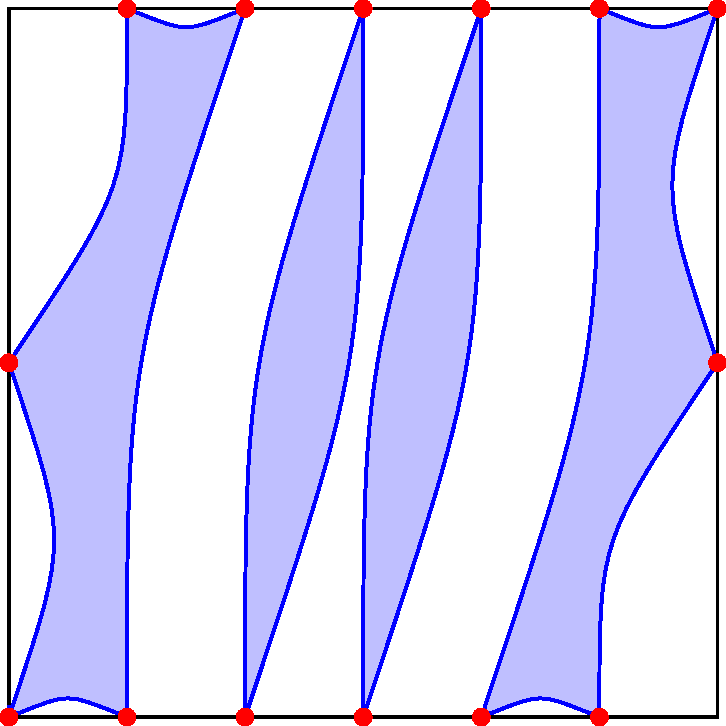
\includegraphics[width=3.075cm]{constr1clear.pdf}};};
\foreach \a in 
    {(20,0), (20,3), (20,6), (20,9)}
    {\draw[line width=0.5mm, black!50] \a rectangle ++(3,3);
    \fill 
        \a++(0.6,1.5) circle (0.2)
        \a++(1.2,1.5) circle (0.2)
        \a++(1.8,1.5) circle (0.2)
        \a++(2.4,1.5) circle (0.2);
        };
\foreach \a in 
    {(20,0), (20,3), (20,6)}
    {\draw[line width=0.7mm]
        \a++(0.6,1.5) -- ++(0,3)
        \a++(0.6,1.5) -- ++(0.6,3)
        \a++(1.2,1.5) -- ++(0.6,3)
        \a++(1.8,1.5) -- ++(0.6,3)
        \a++(2.4,1.5) -- ++(0,3);
    };

\end{tikzpicture}
\end{document}